% ----------------------------------------------------------
\section{Análise dos dados de Dióxido de Nitrogênio}
% ----------------------------------------------------------

\begin{figure}[h]
    \centering
    \caption{Série temporal do sensor NO2-B43F}
    \begin{subfigure}{0.495\textwidth}
        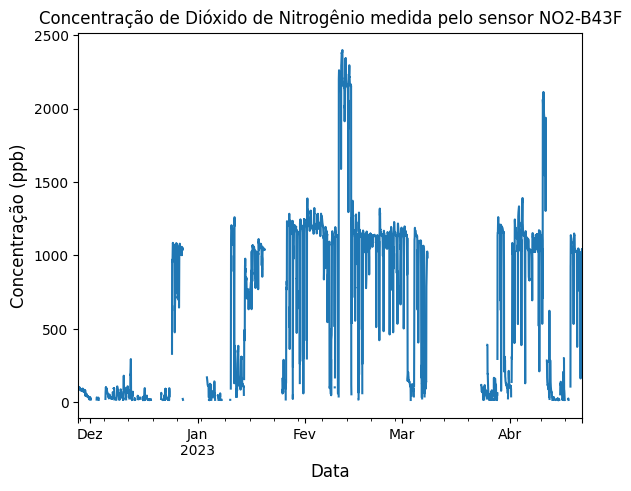
\includegraphics[width=\textwidth]{chapters/3-ANÁLISE DOS DADOS/Figuras/raw-no2-b43f.png}
        \caption{Série temporal do sensor depois de remover valores fora de intervalo}
        \label{fig:data-no2-raw}
    \end{subfigure}
    \hfill
    \begin{subfigure}{0.495\textwidth}
        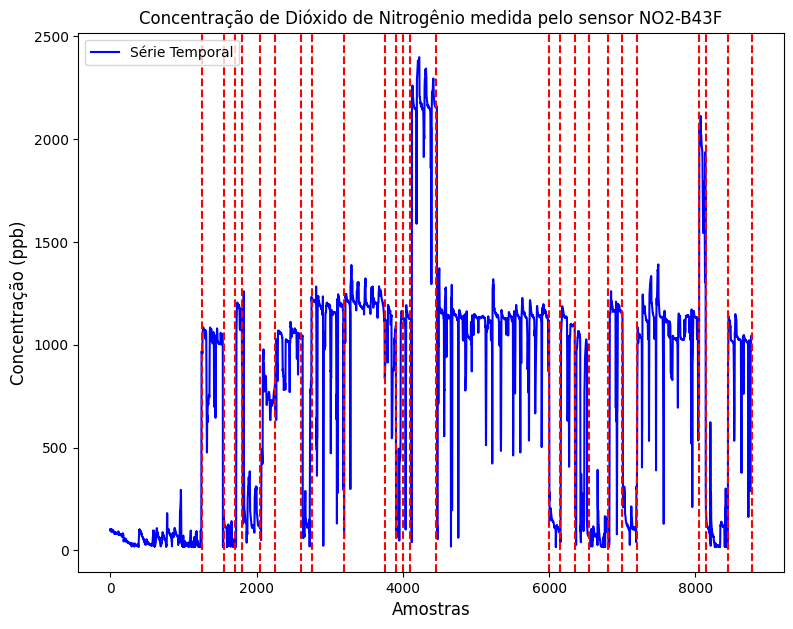
\includegraphics[width=\textwidth]{chapters/3-ANÁLISE DOS DADOS/Figuras/rebase-no2-b43f.png}
        \caption{Pontos de alteração da linha base detectados pelo algoritmo \acrshort{pelt}}
        \label{fig:data-rebase-no2}
    \end{subfigure}
    \hfill
    \label{fig:data-no2-raw-and-pelt}
\end{figure}

A Figura \ref{fig:data-no2-raw} mostra a série temporal do sensor depois de removidos os valores fora de intervalo. Observa-se que a partir do final do mês de dezembro ocorreram seguidas alterações de linha base, detectadas pelo algoritmo \acrshort{pelt}, conforme se ilustra na Figura \ref{fig:data-rebase-no2}. Dado que as mudanças de linha base se mantiveram de forma continuada a partir desse mês, para o restante das análises apenas foram consideradas as leituras anteriores à primeira alteração da linha base do sensor. A Figura \ref{fig:data-no2-preproc-hist} mostra o histograma dos dados das leituras prévias às alterações de linha base, os quais apresentaram uma distribuição log-normal. A Figura \ref{fig:data-co-preproc-1HR} mostra a série temporal das leituras do sensor NO2-B43F após aplicar a metodologia de pré-processamento e re-amostrar os dados para um período de 1 hora.

\begin{figure}[h]
    \centering
    \caption{Histograma das leituras do sensor NO2-B43F}
    \begin{subfigure}{0.45\textwidth}
        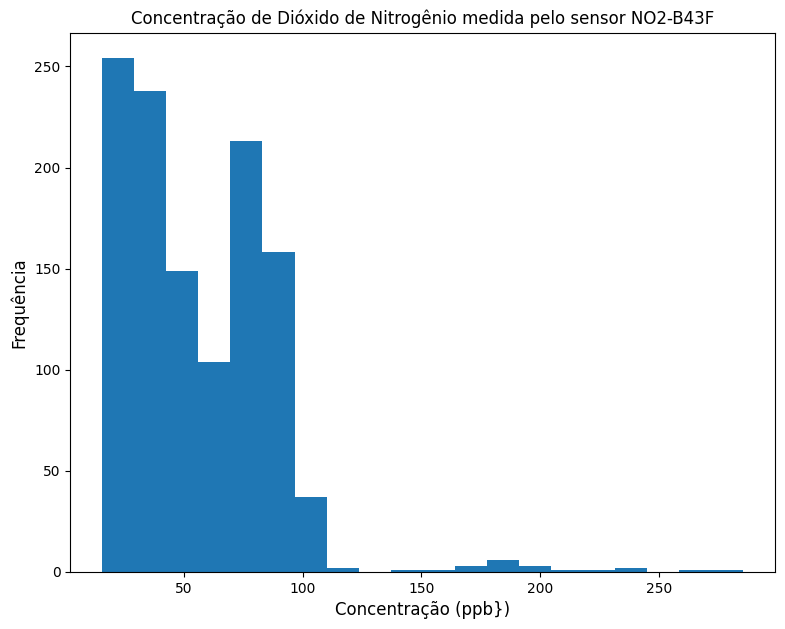
\includegraphics[width=\textwidth]{chapters/3-ANÁLISE DOS DADOS/Figuras/preproc-hist-no2-B43F.png}
        \caption{Histograma após à remoção das alterações de linha base}
        \label{fig:data-no2-preproc-hist}
    \end{subfigure}
    \hfill
    \begin{subfigure}{0.495\textwidth}
        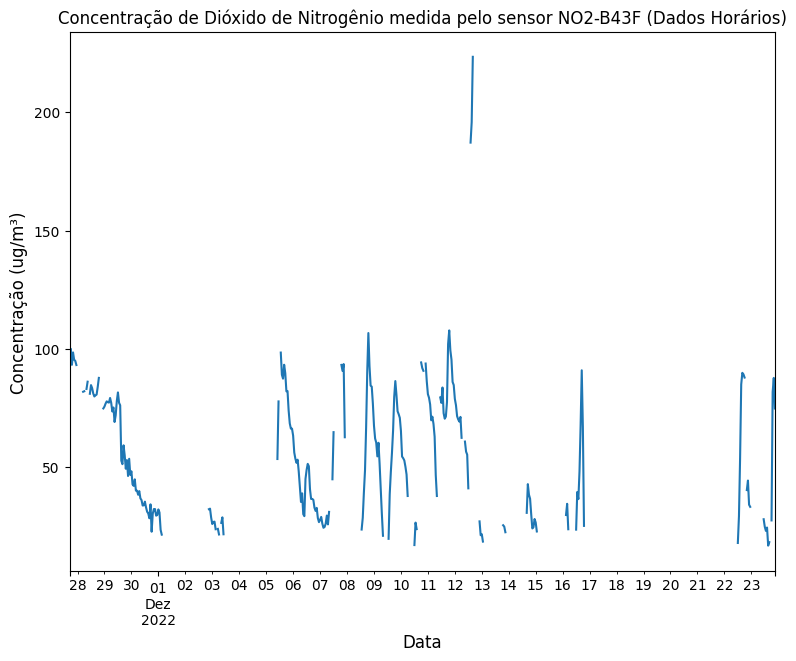
\includegraphics[width=\textwidth]{chapters/3-ANÁLISE DOS DADOS/Figuras/preproc-1HR-no2-B43F.png}
        \caption{Série temporal pré-processada do sensor NO2-B43F com T = 1 hr}
        \label{fig:data-co-preproc-1HR}
    \end{subfigure}
    \label{fig:data-no2-preproc}
\end{figure}

A Figura \ref{fig:data-no2-preproc-box} mostra a série de dados pré-processados do sensor NO2-B43F, juntamente com um gráfico de caixas que representa o comportamento diário das leituras agrupadas por hora do dia. Neste último não é possível perceber um padrão de comportamento muito claro nos dados ao longo do dia, mas em geral observa-se que foram registradas valores de concentração mais altos entre as 14 - 19 hrs. Na Figura \ref{fig:data-no2-reference-box} apresenta-se a série temporal da concentração de referência e seu comportamento diário ao longo do mesmo período. Nas leituras de referência também não é possível observar um padrão diário nos dados.

\begin{figure}[h]
    \centering
    \begin{subfigure}{0.9\textwidth}
        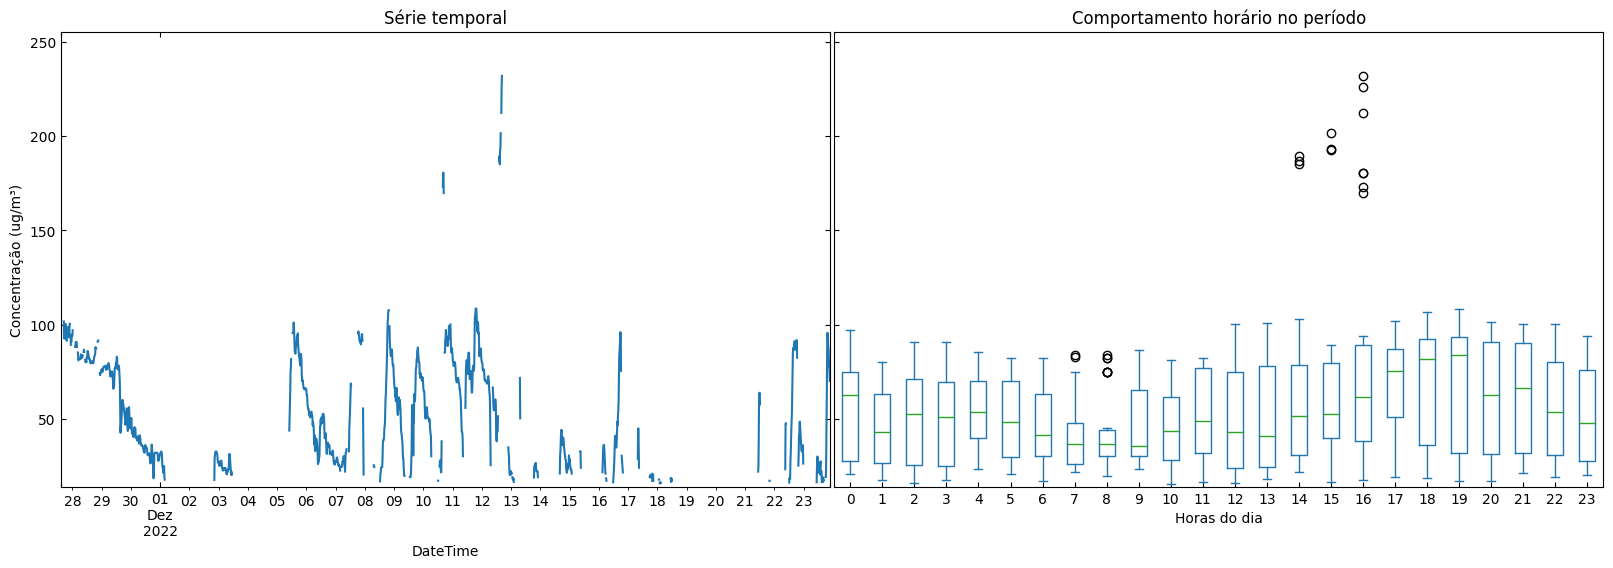
\includegraphics[width=\textwidth]{chapters/3-ANÁLISE DOS DADOS/Figuras/preproc-no2-B43F.png}
        \caption{Série temporal do sensor pré-processada (T = 15 mins) e seu comportamento diário}
        \label{fig:data-no2-preproc-box}
    \end{subfigure}
    \hfill
    \centering
    \begin{subfigure}{0.9\textwidth}
        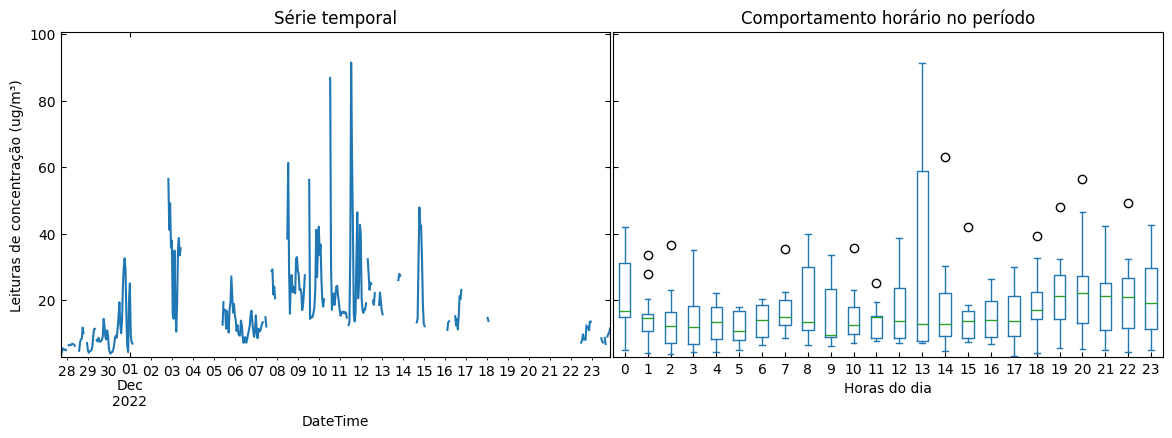
\includegraphics[width=\textwidth]{chapters/3-ANÁLISE DOS DADOS/Figuras/no2-reference-series-and-box.png}
        \caption{Série temporal das leituras de concentração de referência (T = 1 H) e seu comportamento diário}
        \label{fig:data-no2-reference-box}
    \end{subfigure}
    \hfill
    \label{fig:data-no2-box}
\end{figure}

A Tabela \ref{tab:data-contab-no2} mostra a contagem dos dados etiquetados para períodos de 15 minutos e de 1 hora. Observa-se que dos 17647 pontos de dados, que representavam as amostras adquiridas com um período de 15 minutos no intervalo de 20/11/2022 até 23/05/2023, 1175 foram aproveitados como dados válidos, o que representa um 7 \% aproximadamente dos dados originais. Ao re-amostrar esses 1175 pontos em dados horários obtiveram-se 285 amostras horárias de concentração válidas (aproximadamente 45 \% dos dados) para realizar a calibração.

\begin{table}[h]
    \caption{Contabilização das leituras do sensor CO-B4 por etiquetas}
    \centering
    \begin{tabularx}{0.95\textwidth}[h]{
         >{\raggedright\hsize=.475\hsize\arraybackslash}X
         >{\raggedright\hsize=.20\hsize\arraybackslash}X 
         >{\raggedright\hsize=.5\hsize\arraybackslash}X
        | >{\raggedright\hsize=.50\hsize\arraybackslash}X 
         >{\raggedright\hsize=.20\hsize\arraybackslash}X 
         >{\raggedright\hsize=.5\hsize\arraybackslash}X }
        \multicolumn{3}{c|}{Série temporal T = 15 mins} & \multicolumn{3}{c}{Série temporal T = 1 hr} \\
        \hline
        Etiquetas & No. amostras & \% amostras & Etiquetas & No. amostras & \% amostras \\ [0.5ex]
        \hline
        \textit{MISSING} & 5767 & 32.68 \% & \textit{LOWSAMPLES} & 347 & 54.91 \% \\ [0.5ex]
        
        \textit{LTLL} & 2438 & 13.82 \% & \textit{VALID} & 285 & 45.09 \% \\ [0.5ex]
        
        \textit{GTUL} & 0.0 & 0.0 \% & & & \\ [0.5ex]
        
        \textit{STABILIZING} & 673 & 3.81 \% & & & \\ [0.5ex]
        
        \textit{BADSPIKE} & 1 & 0.01 \% & & & \\ [0.5ex]
        
        \textit{LTQTLE01} & 32 & 0.18 \% & & & \\ [0.5ex]
        
        \textit{GTQTLE99} & 36 & 0.20 \% & & & \\ [0.5ex]
        
        \textit{REBASE} & 7525 & 42.64 \% & & & \\ [0.5ex]
        
        \textit{VALID} & 1175 & 6.66 \% & & & \\ [0.5ex]
        \hline
        TOTAL & 17647 & & TOTAL & 632 & \\
    \end{tabularx}
    \label{tab:data-contab-no2}
\end{table}

\subsection{Dependência com a temperatura}

Investigou-se a existência de correlação entre as leituras do sensor de \acrshort{no2} e as variações de temperatura medida no interior da câmara de medição. Para tal, foram empregados os testes estatísticos de correlação de Spearman e Kendall. Os resultados desses testes revelaram coeficientes de correlação baixos. O coeficiente de Spearman calculado foi de 0.09, com um valor de p inferior a 0.5. De maneira semelhante, o coeficiente de Kendall foi de 0.06, também com p < 0.05. Ao avaliar a hipótese nula de ausência de correlação, os resultados forneceram evidências robustas para sua rejeição, sugerindo que existe correlação, embora baixa, entre as leituras do sensor de \acrshort{no2} e as variações de temperatura. A Figura \ref{fig:data-temp-no2-corr} mostra um gráfico de dispersão entre os dados do sensor e a temperatura, ilustrando os resultados de correlação obtidos. As leituras de referência mostraram um comportamento diferente, não apresentando correlação com a variável temperatura. Os testes estatísticos de Spearman e Kendall mostraram que não foi possível rejeitar a hipótese nula de não existência de correlação entre as variáveis (Figura \ref{fig:data-temp-no2-ref-corr}).

\begin{figure}[h]
    \centering
    \caption{Relação dos dados de concentração de \acrshort{no2} com a temperatura}
    \begin{subfigure}{0.5\textwidth}
        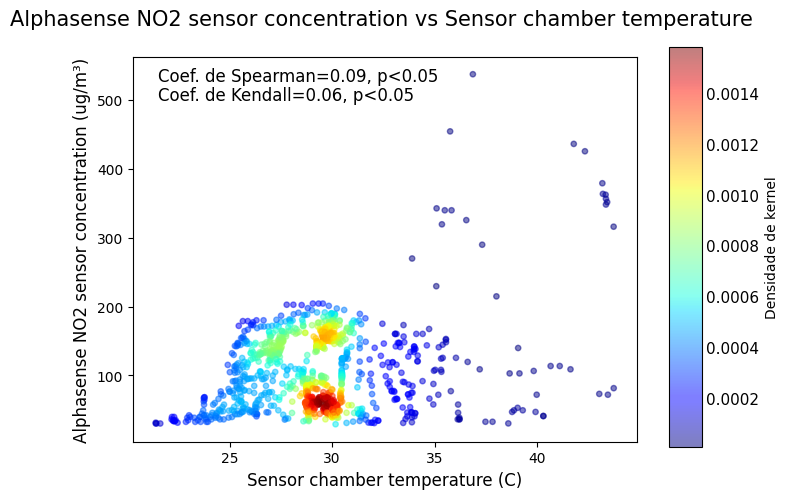
\includegraphics[width=\textwidth]{chapters/3-ANÁLISE DOS DADOS/Figuras/temperature-no2-B43F.png}
        \caption{Relação entre as leituras do sensor NO2-B43F (\(\mu g/m^3\)) e a temperatura (\textdegree C)}
        \label{fig:data-temp-no2-corr}
    \end{subfigure}
    \hfill
    \begin{subfigure}{0.48\textwidth}
        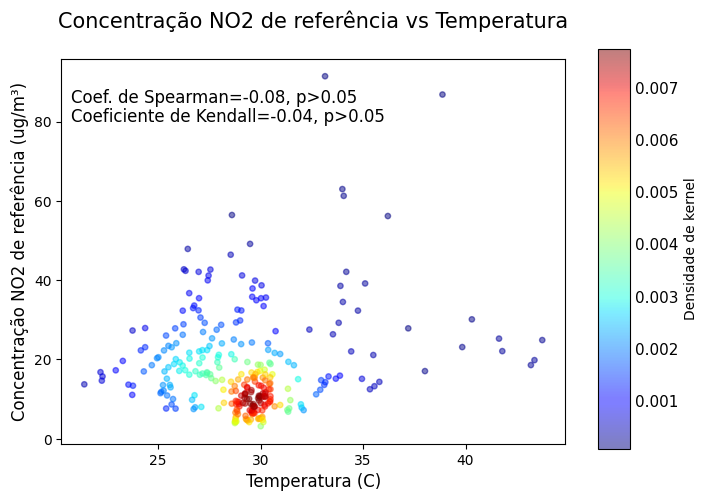
\includegraphics[width=\textwidth]{chapters/3-ANÁLISE DOS DADOS/Figuras/temperature-no2-reference.png}
        \caption{Relação entre os valores de concentração de referência (\(\mu g/m^3\)) e a temperatura (\textdegree C)}
        \label{fig:data-temp-no2-ref-corr}
    \end{subfigure}
    \hfill
    \label{fig:data-no2-temp}
\end{figure}

\subsection{Comparação das leituras de \acrshort{no2} do sensor NO2-B43F com as medições de referência}

Nas Figuras \ref{fig:data-no2-reference-time-series} e \ref{fig:data-no2-reference-corr} apresentam-se as leituras de \acrshort{no2} obtidas pelo sensor NO2-B43F de Alphasense e a estação de referência. Observa-se que as leituras do sensor superestimaram os valores de concentração de referência com valores aproximadamente 5 vezes maiores. Os testes de Spearman e Kendall revelaram que não foi possível rejeitar a hipótese nula de que não existe correlação entre os dados do sensor e da estação de referência.

\begin{figure}[h!]
    \centering
    \caption{Séries temporais e gráficos de dispersão das medições de \acrshort{no2}}
    \begin{subfigure}{0.49\textwidth}
        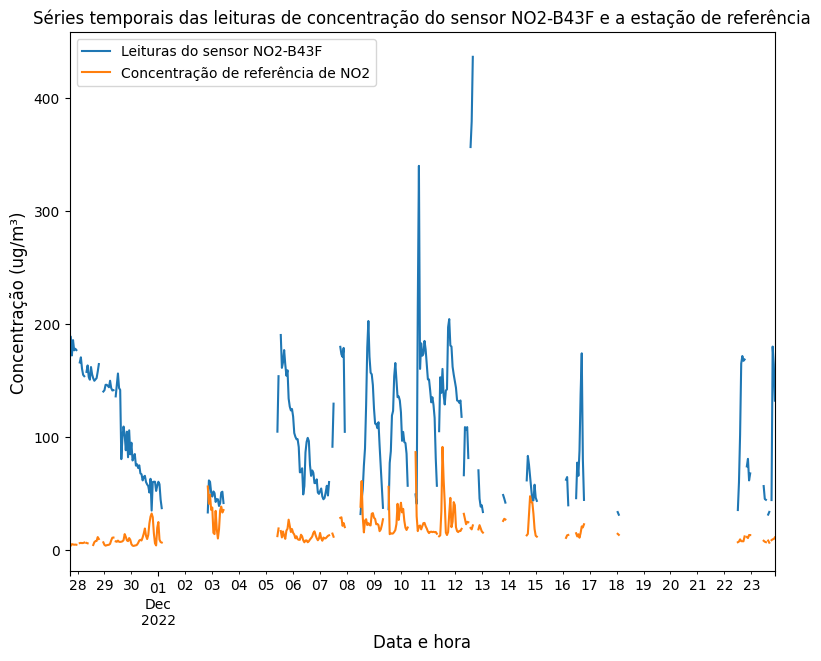
\includegraphics[width=\textwidth]{chapters/3-ANÁLISE DOS DADOS/Figuras/no2-b43F-reference-time-series.png}
        \caption{Séries temporais das leituras de \acrshort{no2} do sensor NO2-B43F e a estação de referência}
        \label{fig:data-no2-reference-time-series}
    \end{subfigure}
    \hfill
    \begin{subfigure}{0.48\textwidth}
        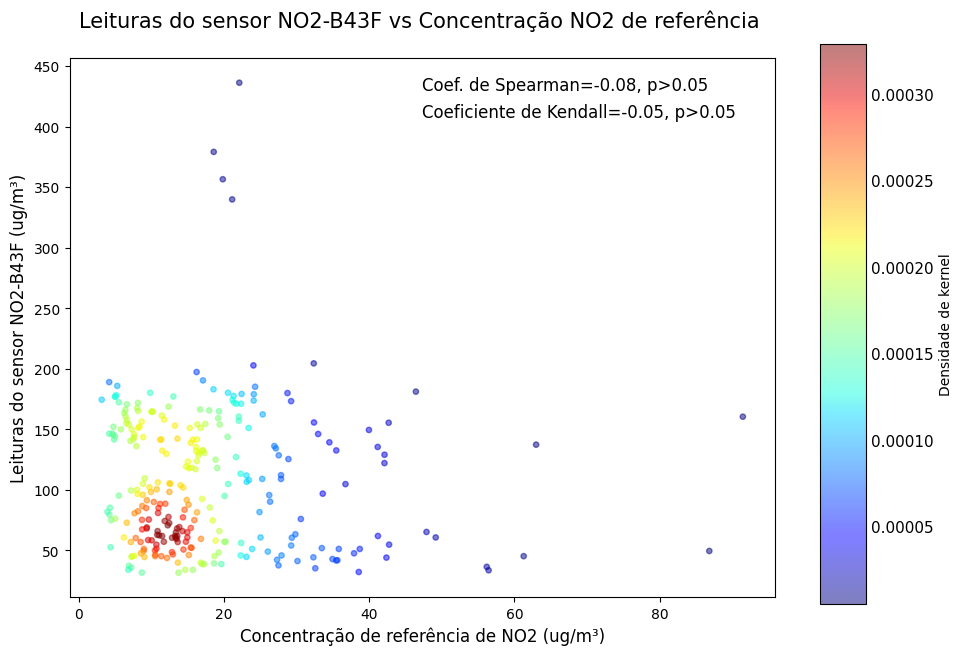
\includegraphics[width=\textwidth]{chapters/3-ANÁLISE DOS DADOS/Figuras/no2-b43F-reference-correlation.png}
        \caption{Gráfico de dispersão das leituras de \acrshort{no2} do sensor NO2-B43F e a estação de referência}
        \label{fig:data-no2-reference-corr}
    \end{subfigure}
\end{figure}